\documentclass[12pt]{exam}  % exam document class - MIT Mathematics
\usepackage[utf8]{inputenc}

\usepackage{tikz}
\usepackage{pgfplots}

\usetikzlibrary{math}
%\usetikzlibrary{datavisualization.formats.functions}
%\usetikzlibrary{datavisualization}
\usetikzlibrary{intersections}
\pgfplotsset{compat=1.16}


\usepackage{xcolor}
\usepackage{colortbl}
\usepackage{amsmath}
\usepackage{amssymb}
\usepackage{gnuplottex}
\usepackage{graphicx}
\usepackage{siunitx}
\usepackage{multicol}
\usepackage{tasks}
\usepackage{physics}
\usepackage{cancel}
\usepackage{todonotes}
\usepackage{romannum}

\renewcommand{\solutiontitle}{\noindent\textbf{Lösung:}\par\noindent}

\renewcommand{\questionshook}{%
\setlength{\leftmargin}{0pt}%
\setlength{\labelwidth}{-\labelsep}%
}

\newcommand{\uuline}[1]{\underline{\underline{~#1~}}}

\setlength{\jot}{8pt}

\settasks{
    label-width = 11.0971pt
  }


%%%%%%%%% Ausgabe der Lösungen %%%%%%%%%

%\noprintanswers
\printanswers

%%%%%%%%% Rahmen um Lösung %%%%%%%%%
\unframedsolutions
%\framedsolutions

\begin{document}
		\pagestyle{headandfoot}

\firstpageheader{Übungsaufgaben\\ Bodendynamik}{TU Bergakademie Freiberg \\Institut für Geotechnik}{Seite \thepage\ von \numpages\\}
\firstpageheadrule

\firstpagefooter{}{}{}
\runningfooter{}{}{}

\runningheader{Übungsaufgaben\\ Bodendynamik}{TU Bergakademie Freiberg \\Institut für Geotechnik}{Seite \thepage\ von \numpages\\}
\runningheadrule
\runningfootrule

\setlength{\jot}{8pt}


%%% Todonotes margin - remove when done
\setlength {\marginparwidth }{2cm}
		\tikzset{
%DKspring(length) length=2...10
DKspring/.pic={
\coordinate (half_up) at (0.5*0.125*#1-0.5*0.125*2, 0.5*0.125*10-0.5*0.125*#1); %at (0.5*(#1-0.2), 0.5*(1.0-#1));
\coordinate (full_up)   at ( 0.125*#1-    0.125*2,     0.125*10-    0.125*#1);
\coordinate (full_down) at ( 0.125*#1-    0.125*2,    -0.125*10+    0.125*#1);
\draw (0, 0) -- ++(1, 0) -- ++(half_up)
    -- ++(full_down) -- ++(full_up) 
    -- ++(full_down) -- ++(full_up)
    -- ++(full_down) -- ++(full_up)
    -- ++(full_down) -- ++(half_up)
    -- ++(1, 0);
    },   
%DKdashpot(length) length=02...10    
DKdashpot/.pic={
\coordinate (upper_end) at (#1-0.5, 0.5);
\coordinate (lower_end) at (#1-0.5,-0.5);
\coordinate (upper_pos) at (#1-1, 0.5);
\coordinate (lower_pos) at (#1-1,-0.5);
\coordinate (center_pos) at (#1-1, 0.0);
\coordinate (center_end) at (#1, 0.0);
\draw (0, 0) -- ++(1, 0);
\draw (upper_end) -- (1, 0.5) -- (1, -0.5) -- (lower_end);
\draw (center_pos) -- (center_end);
\draw (upper_pos) -- (lower_pos);
    },
DKbase/.pic={
\draw[thick] (0, 1.5) -- (0, -1.5);
\foreach \y in {-1.5,-1.0,...,1.0} \draw[thin] (0, \y) -- +(-0.5, 0.5);
},
 invisible/.style={opacity=0},
  visible on/.style={alt={#1{}{invisible}}},
  alt/.code args={<#1>#2#3}{%
    \alt<#1>{\pgfkeysalso{#2}}{\pgfkeysalso{#3}} % \pgfkeysalso doesn't change the path
  }
}

	\begin{coverpages}
		\huge\centering Übungsaufgaben Bodendynamik - SS \the\year 
		\normalsize
	\end{coverpages}
	
	\begin{questions}
	
		\section{Einleitung}
		%\fullwidth{\Large \textbf{Essay questions}}
		\question{Recherche}   
Suchen Sie nach Nachrichten mit Geotechnikbezug.

\begin{solution}
Der Weg ist das Ziel 
\end{solution}

%%%%%%%%%%%%%%%%%%%%%%%%%%%%%%%%%%%%%%%%%%%%%%%%%%%%%%%%%%%%%%%%%%%%%%%%%%%%%%

\question{Online--Ressourcen}
Suchen Sie nach Videos und interaktivem Material zu geotechnischen Schlagwörtern.

\begin{solution}
Der Weg ist das Ziel 
\end{solution}

		
		\newpage
		\section{Grundlagen}
		   \subsection{Einfreiheitsgradschwingungen}
		   \question{Erzwungene, ungedämpfte Schwingung}
\vspace{1em}

\begin{minipage}[t]{.49\linewidth}
geg.:
\begin{tasks}(2)
    \task[] $m = \SI{3}{\kilo\gram}$
    \task[] $k = \SI{10}{\newton\per\meter}$
    \task[] $F(t) = \hat{F} \sin{\omega t}$
    \task[] $\hat{F} = \SI{5}{\newton}$
    \task[] $\omega = \SI{10}{\radian\per\second}$
    \task[] $t=\SI{0}{\second}$
    \task[] $u_0 = \SI{0.1}{m}$
    \task[] $\dot{u}_0 = \SI{0}{\meter\per\second}$
\end{tasks}
\end{minipage}
\begin{minipage}[t]{.49\linewidth}
ges.:
\begin{tasks}
    \task $u(t)$
\end{tasks}
\end{minipage}

\begin{solution}
    \begin{alignat*}{2}
        &(c = \SI{0}{\newton\second\per\meter}, F_C = \SI{0}{\newton}, F_S = \hat{F} = \SI{5}{\newton})\\
        &\omega_0 = \sqrt{k/m} &&= \SI{1.826}{\radian\per\second} \\
        &\zeta = \frac{c}{2\sqrt{mk}} &&= 0 \\
        &\eta = \omega/\omega_0 &&= 5.477\\
        &V = (1-\eta^2)^{-1} &&=  0.0345 \\
        &u_C = -2V^2\zeta\eta\hat{F}/k &&= \SI{0}{\meter} \\
        &u_S = V^2(1-\eta^2)\hat{F}/k &&= \SI{-0.0172}{\meter}
    \end{alignat*}

    \begin{align*}
        u_0 &= C_1 + u_C \\
        \dot{u}_0 &= \omega_0 C_2+\omega u_S\\
        &\rightsquigarrow \\
        C_1 &=  u_0 - U_C = \SI{0.1}{\meter}\\
        C_2 &= \frac{\dot{u}_0 - \omega u_S}{\omega_0} = \SI{0.0944}{\meter} \\
        \vspace{1cm}
    \end{align*}

    \begin{equation*}
        \begin{split}
            u(t) = \SI{0.1}{\meter} \cos{(\SI{1.826}{\radian\per\second} t)} +\SI{0.0944}{\meter} \sin{((\SI{1.826}{\radian\per\second} t))} \\ - \SI{0.0172}{\meter}\sin{(\SI{10}{\radian\per\second} t)}
        \end{split}
    \end{equation*}
        \fbox{\textbf{Anmerkung:} Das Einschwingen dauert im  ungedämpften Fall unendlich lang.}
\end{solution}
    
    
%%%%%%%%% Übungsaufgabe 2 %%%%%%%%%

\question{Erzwungene, gedämpfte Schwingung}

    \begin{minipage}[t]{.49\linewidth}
        geg.:
        \begin{tasks} (2)
           \task[] $m = \SI{3}{\kilo\gram}$
           \task[] $c = \SI{1}{\newton\second\per\meter}$
           \task[] $k = \SI{10}{\newton\per\meter}$
            \task[] $F(t) = \hat{F} \sin{\omega t}$
           \task[] $\hat{F} = \SI{5}{\newton}$
           \task[] $\omega = \SI{10}{\radian\per\second}$
           \task[] $t=\SI{0}{\second}$
           \task[] $u_0 = \SI{0.1}{m}$
           \task[] $\dot{u}_0 = \SI{0}{\meter\per\second}$
           \task[] $t_0 = \SI{0}{\second}$
        \end{tasks}
        \end{minipage}
        \begin{minipage}[t]{.49\linewidth}
        ges.:
        \begin{tasks}
            \task[] $u(t)$
        \end{tasks}
    \end{minipage}\\
    \vspace{1cm}

    \underline{Zusatzfrage:} Wie ändert sich die Lösung, wenn die Anregung zusätzlich einen Konstantanteil enthält $F(t) = F_{DC} +\hat{F} \sin{(\omega t)}$ (Stichwort \textit{statische Ruhelage})?

    \begin{solution}
        \begin{alignat*}{2}
            &\omega_0 = \sqrt{k/m} &&= \SI{1.826}{\radian\per\second} \\
            &\zeta = \frac{c}{2\sqrt{mk}} &&= 0.091 \\
            &\eta = \omega/\omega_0 &&= 5.477\\
            &V = \frac{1}{\sqrt{(1 - \eta^2)^2 + (2\zeta\eta)^2}} &&= 0.034\\
            &\text{da: } a(t) = \frac{F(t)}{k} \sin(\omega t) = \hat{a} \cos(\psi_a) \cos(\omega t) + \hat{a} \sin{\psi_a} \sin{\omega t} \\
            &F_c = 0 && F_s = \SI{5}{\newton} \\
            &a_c = \frac{F_c}{k} &&= \SI{0}{\newton}\\ 
            &a_s = \frac{F_s}{k} &&= 0.2 m^{-1} \\
            &a= a_c \sin(\omega t) + a_s \sin(\omega t) &&= 0 \\
            &\psi = \arctan(\frac{2\zeta \eta}{1-\eta^2}) &&= \SI{3.107}{\radian}\\
            &u_c = V^2((1-\eta^2)a_c - 2 \zeta \eta a_s) &&= \SI{-0.0006}{\meter}\\
            &u_s = V^2((1 - \eta^2)a_s + 2 \zeta \eta a_c) &&= \SI{-0.0172}{\meter}\\
            &u_p(t)= u_c \cos(\omega t) + u_s \sin(\omega t) &&= \\
        \end{alignat*}
    \end{solution}
        
\begin{figure}[h]
    \centering
    \begin{gnuplot}[terminal=epslatex, terminaloptions={size 15cm,5cm}]
       set zeroaxis
       unset border
       set xtics axis
       unset ytics
       unset key

       set xr [0:3*pi]
       set yr [-1:1]
       set xl "t" offset 27,7,0
       set yl "u" offset 2,6,0 rotate by 0

       set xtics ("$t_{max1}$" pi/4, "$t_{max2}$" pi/4+2*pi)

       set label 1 "" at pi/4,1 point pointtype 7 pointsize 2 lc 0
       set label 2 "" at pi/4+2*pi,1 point pointtype 7 pointsize 2 lc 0

       set arrow 1 from 0,0 to graph 0, first 1 filled head
       set arrow 2 from 0,0 to first 0, graph 0 filled head
       set arrow 3 from 0,0 to graph 1,.5 filled head

       plot cos(x-pi/4) w l lc 0
    \end{gnuplot}
\end{figure}


\question{Ausschwingversuch}

    \begin{minipage}[t]{.49\linewidth}
        geg.:
        \begin{tasks}(1)
           \task[] $m = \SI{3}{\kilo\gram}$
           \task[] $u(t_{max1}) = \SI{0.10}{\meter}$
           \task[] $u(t_{max2}) = \SI{0.08}{\meter}$
           \task[] $T_{id} = t_{max2}-t_{max1} = 1$
           \task[] $N = 1$
        \end{tasks}
        \end{minipage}
        \begin{minipage}[t]{.49\linewidth}
        ges.:
        \begin{tasks}
            \task $c ~,~ k$
        \end{tasks}
    \end{minipage}\\
    \vspace{1cm}

    \fbox{\underline{Hinweis:} Nutzen Sie das logarithmische Dekrement $\Lambda = \log \frac{u(t_{max1})}{u(t_{max2})}$ als Zwischenergebnis.}

    \begin{solution}
        \begin{alignat*}{2}
            &\omega_{1_{id}} = \frac{2 \pi}{T_{id}} &&= 2 \pi\\
            &\Delta_{id} = \frac{1}{N \cdot T_{id} } \cdot \ln{\frac{u_1}{u_2}} &&= \text{??}\\
            &c_{id} = 2 \cdot \Delta_{id} \cdot m &&= \SI{1.339}{\newton \second \per \meter}\\
            &\omega_{0_{id^2}} = \omega_{1_{id}}^2 + \Delta_{id}^2 &&= \\
            &k_{id} = \omega_{0_{id^2}} \cdot m &&= \\
        \end{alignat*}
    \end{solution}

     %%%%%%%%% Übungsaufgabe 4 %%%%%%%%%

 \question{Schwingsaitenwaage}



\begin{minipage}[t]{.49\linewidth}
    geg.:
    \begin{tasks}(1)
        \task[] $m = \SI{3}{\kilo\gram}$
        \task[] $\omega_{measured} = \SI{10}{\radian\per\second}$
        \task[] $0 < \zeta < 1$
        \task[] $\zeta_{measured} = 0.1$
    \end{tasks}
    \end{minipage}
    \begin{minipage}[t]{.49\linewidth}
    ges.:
    \begin{tasks}
        \task $k$
    \end{tasks}
\end{minipage}\\
\vspace{1cm}

\underline{Zusatzfrage:} Je nach Messprinzip, wird entweder die ungedämpfte
Eigenfrequenz, die gedämpfte Eigenfrequenz oder die maximale Anwortamplitude
hervorrufende Anregungsfrequenz direkt erfasst. Wie groß ist für $\zeta = 0.1$ der
Fehler bei der Schätzung von $k$, wenn man diese Frequenzen gleichsetzt?

\begin{solution}
    \begin{alignat*}{2}
        &\text{ungedämpfte Eigenkreisfrequenz  } \omega_0 = \sqrt{\frac{k}{m}} \\
        &k_{ungedämpft} = m \cdot \omega_{measured}^2 &&= \SI{300000}{\newton \per \meter} \\
        &\text{gedämpfte Eigenfrequenz  } \omega_1 = \omega_0 \sqrt{1-\zeta^2} \\
        &\omega_{gedämpft} = \frac{\omega_{measured}}{\sqrt{1-\zeta_{measured}^2}} &&= \\
        &k_{gedämpft} = m \cdot \omega_{gedämpft}^2 &&= \SI{303030}{\newton \per \meter}\\
        &\Delta = 100 \cdot \frac{|k_{gedämpft} - k_{ungedämpft}|}{k_{ungedämpft}} &&= 1.01 \%\\
        &\text{maximale Antwortamplitude bei der Anregungsfrequenz  } \omega_{MA} = \omega_0 \sqrt{1-2 \zeta^2} \\
        &\omega_{MA} = \frac{\omega_{measured}}{\sqrt{1-\zeta_{measured}^2}} &&= \\
        &k_{MA} = m \cdot \omega_{MA}^2 &&= \SI{306122}{\newton \per \meter}\\
        &\Delta = 100 \cdot \frac{|k_{MA} - k_{ungedämpft}|}{k_{ungedämpft}} &&= 2.04 \% \\ 
    \end{alignat*}
\end{solution}



		   \subsection{Frequenzanalyse}
		   \question{Berechnen Sie die Antwort des gedämpften Einmassenschwingers aus Aufgabe 2 TODO fix reference
(letzte Übung) auf das Sägezahnsignal $(T = \SI{1}{\second}, u_{\max} = - u_{\min} = \SI{0.1}{\meter})$,
welches durch eine Fourierreihe bis $N = 2$ approximiert werden soll. Als
Anfangsbedingungen gelten: $u(-T/2) = \SI{0}{\meter}, \dot{u}(-T/2) = \SI{0}{\meter\per\second}
$.}

\begin{minipage}[c]{.49\linewidth}
 \begin{align*}
     a(t) = \frac{2a_{\max}}{T}t -nT \\
     nT - \frac{T}{2} < t \leq nT + \frac{T}{2}
 \end{align*}
 \end{minipage}
     
     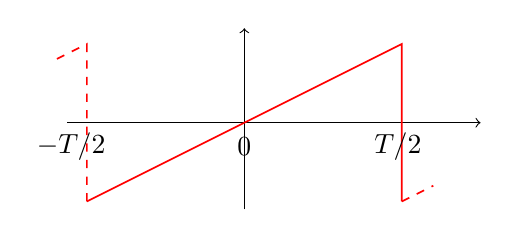
\begin{tikzpicture}[baseline=0mm] 
\draw[->] (-2.25, 0) -- (3, 0);
\draw[->] ( 0,-1.1) -- (0, 1.2);
\draw[semithick,red] (-2,-1) -- ( 2, 1) -- (2,-1);
\draw[semithick,red, dashed] (-2,-1) -- (-2, 1) -- (-2.4, 0.8);
\draw[semithick,red, dashed] ( 2,-1) -- ( 2.4,-0.8);
\draw (-2.2,-0.3) node {$-T/2$};
\draw ( 0,-0.3) node {$0$};
\draw ( 1.95,-0.3) node {$T/2$};
\end{tikzpicture}


\begin{solution}
\begin{minipage}[c]{.49\linewidth}
 \begin{align*}
     a(t) &= ct \\
     c &= \frac{2a_{\max}}{T} \\
     \tilde{w}_k &= \frac{2\pi k}{T}
 \end{align*}
\end{minipage}

 \textbf{\raggedright Darstellung der Anregung als Fourierreihe ($N=2$)}

\vspace{1em}

\begin{align*}
    \intertext{\flushleft Benötigte Integrale:}
    \int x \sin(ax) \dd{x} &= \frac{\sin(ax) - x \cos(ax)}{a} \\
    \int x \cos(ax) \dd{x} &= \frac{\cos(ax) + x \sin(ax)}{a}
\end{align*}

\dotfill

\begin{align*}
    A_0 &=  \frac{2}{T} \int\limits_{-\frac{T}{2}}^{\frac{T}{2}} a(t)\dd{t} = \frac{2}{T} \int\limits_{-\frac{T}{2}}^{\frac{T}{2}} ct \dd{t} = \frac{2}{T} \,\Big|\, \frac{c}{2}t^2\,\Big|_{t = -\frac{T}{2}}^{\frac{T}{2}} = \uuline{0}\\
    A_k &= \frac{2}{T} \int\limits_{-\frac{T}{2}}^{\frac{T}{2}} a(t) \cos(\overbrace{\frac{2\pi k}{T}}^{\tilde{w}_k}t)\dd{t} = \frac{2}{T} \int\limits_{-\frac{T}{2}}^{\frac{T}{2}} ct \cos(\tilde{w}_k t) \dd{t} \\
    &= \frac{2}{T} \,\Big|\,\frac{c}{\tilde{w}_k} (\cos(\tilde{w}_k t) + t \sin(\tilde{w}_k t))\,\Big|_{t = -\frac{T}{2}}^{\frac{T}{2}} = \uuline{0}
\end{align*}


\begin{minipage}[t]{.49\linewidth}

      $\cos(\tilde{w}_k t)$\\

    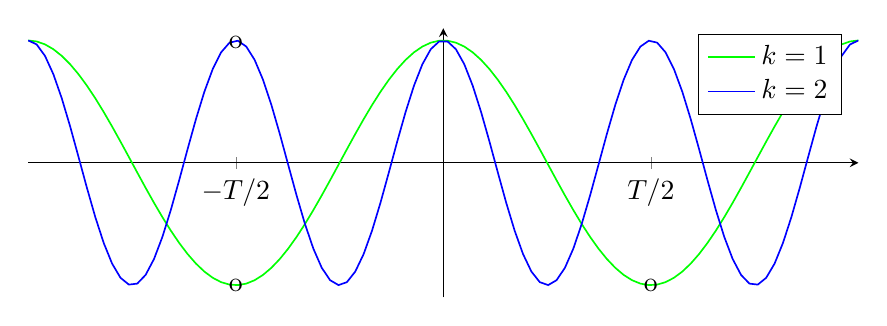
\begin{tikzpicture}
    \begin{axis}[
        width = \linewidth,
        height = 5cm,
        axis x line=center,
        axis y line=middle,
        samples=100,
        ymin=-1.1, ymax=1.1,
        xmin=-pi, xmax=pi,
        ytick=\empty,
        xtick={-pi/2,pi/2},
        xticklabels={$-T/2$,$T/2$}
        ]
        \addplot [semithick, green, domain=-pi:pi] {cos(2*deg(x))};
        \addlegendentry{$k=1$};
        \addplot [semithick, blue, domain=-pi:pi] {cos(4*deg(x))};
        \addlegendentry{$k=2$};
        \draw (axis cs: -1.57,0.98) node {o};
        \draw (axis cs: -1.57,-1) node {o};
        \draw (axis cs:  1.57,-1) node {o};
    \end{axis}
\end{tikzpicture}

\end{minipage}
\begin{minipage}[t]{.49\linewidth}

    $\sin(\tilde{w}_k t)$\\

    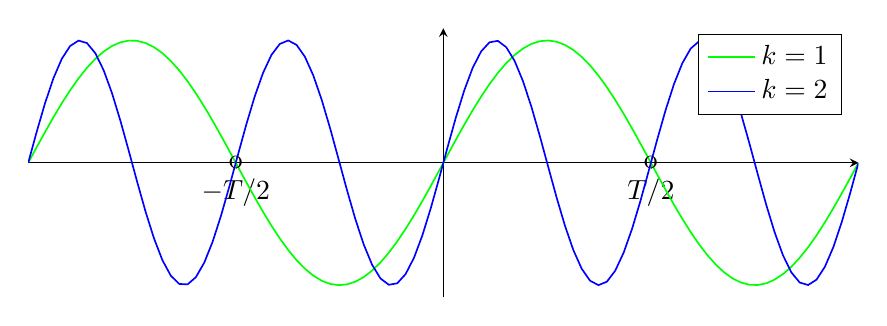
\begin{tikzpicture}
    \begin{axis}[
        width = \linewidth,
        height = 5cm,
        axis x line=center,
        axis y line=middle,
        samples=100,
        ymin=-1.1, ymax=1.1,
        xmin=-pi, xmax=pi,
        ytick = \empty,
        xtick={-pi/2,pi/2},
        xticklabels={$-T/2$,$T/2$}
        %legend style={draw=none}
        ]
        \addplot [semithick, green, domain=-pi:pi] {sin(2*deg(x))};
        \addlegendentry{$k=1$};
        \addplot [semithick, blue, domain=-pi:pi] {sin(4*deg(x))};
        \addlegendentry{$k=2$};
        \draw (axis cs: -1.57,0) node {o};
        \draw (axis cs:  1.57,0) node {o};
    \end{axis}
\end{tikzpicture}

\end{minipage}
\vspace{1em}

\begin{align*}
     B_k &= \frac{2}{T} \int\limits_{-\frac{2}{T}}^{\frac{2}{T}} ct \sin(\tilde{w}_k t) \dd{t} = \frac{2}{T}\,\Big|\, \frac{c}{\tilde{w}_k}(\sin(\tilde{w}_k t)-t\cos(\tilde{w}_k t))\,\Big|_{t={-\frac{2}{T}}}^{t=\frac{2}{t}} \\
     &= \frac{-2c}{\tilde{w}_k} \cos(\tilde{w}_k\frac{T}{2}) =
     \left\{
     \begin{array}{lll}
     \cfrac{2c}{\tilde{w}_k} & &k = 1,3,5,\dots\\[1em]
     -\cfrac{2c}{\tilde{w}_k} & &k = 2,4,6,\dots
     \end{array}\right.
\end{align*}

\begin{align*}
     \begin{array}{lcl}
        a = \overbrace{B_1\sin(\tilde{w}_1 t)}^{a_1(t)} + \overbrace{B_1\sin(\tilde{w}_2 t)}^{a_2(t)} & \rightsquigarrow & u_p(t) = u_{p1}(t) + u_{p2}(t) \\[1em]
        B_1 = \cfrac{4a_{\max}\cancel{T}}{2\pi\cancel{T}} \qquad \tilde{w}_1 = \cfrac{2\pi}{T} && u_{p1}^{(t)} = u_{C1} \cos(\tilde{w}_1 t) + u_{S1} \sin(\tilde{w}_1 t) \\[1em]
        B_2 = \cfrac{4a_{\max}}{4\pi} \qquad \tilde{w}_2 = \cfrac{4\pi}{T}&& \underbrace{u_{p2}^{(t)} = u_{C2} \cos(\tilde{w}_2 t) + u_{S2} \sin(\tilde{w}_2 t)} \\
        &&\text{Partikuläre Lösung - siehe Übung}\\
        &&\text{harmonisch erregter Einmassenschwinger}
    \end{array}
\end{align*}\\[2em]

\textbf{Anpassung der Gesamtlösung an die Anfangsbedingungen}
    
    Die Gesamtlösung setzt sich additiv aus der Lösung der homogenen Gleichung und der bereits bestimmten Partikulärlösung zusammen
    \begin{align*}
        u(t) &= C_1\cos(\omega_1 t)e^{-\delta t} + C_2 \sin(\omega_1 t)e^{-\delta t} + u_p(t),\\
        \dot{u}(t) &= -C_1 \exp(-\delta t) \cdot (\omega_1 \sin(\omega_1 t) + \delta \cos(\omega_1 t)) + C_2 \exp(-\delta t) \cdot (\cos(\omega_1 t) + \sin(\omega_1 t)) + \dot{u_p}(t).
    \end{align*}
    Mit den Anfangsbedingungen
    \begin{align*}
        u(t_0) &= u_0 \\
        \dot{u}(t_0) &= \dot{u}_0
    \end{align*}
    liegen zwei Gleichungen mit zwei Unbekannten vor
    \begin{align*}
    \begin{bmatrix}
        A_{11} & A_{12}\\
        A_{21} & A_{22}
    \end{bmatrix}
    \begin{bmatrix}
        C_1 \\
        C_2
    \end{bmatrix}
    &=
    \begin{bmatrix}
    b_1 \\
    b_2
    \end{bmatrix} \\
    \intertext{mit}
        A_{11}&= -\omega_1 \sin(\omega_1 t) \exp(-\delta t),\\
        A_{12}&= - \delta \cos(\omega_1 t) \exp(-\delta t),\\
        A_{21}&= \cos(\omega_1 t) \exp(-\delta t),\\
        A_{22}&= \sin(\omega_1 t) \exp(-\delta t),\\
        b_{1}&= -u_{C_1} \tilde{\omega_1} \sin(\tilde{\omega_1}t) + u_{S_1} \tilde{\omega_1} \cos(\tilde{\omega_1}t),\\
        b_{2}&= -u_{C_2} \tilde{\omega_2} \sin(\tilde{\omega_2}t) + u_{S_2} \tilde{\omega_2} \cos(\tilde{\omega_2}t).
    \end{align*}

    \begin{solution}  
        \begin{align*}
            t_0 &= \SI{0.5}{\second}\\
            T_a &= \SI{9}{\second} \\
            k &=  \SI{10}{\newton \per \second} \\
            c &= \SI{1}{\newton \second \per \meter} \\
            a_{C_1} &= 0 \\
            a_{S_1} &= 1 \\
            \omega &= \frac{2 \pi}{T_a} &&= 0.698 \\
            \omega_0 &= \sqrt{\frac{k}{m}} &&= 1.826\\
            \zeta &= \frac{c}{2 \sqrt{km}} &&= 0.091\\
            \eta &= \frac{\omega}{\omega_0} &&= 0.382\\
            V &= \frac{1.0}{\sqrt{{(1-\eta^2)}^2 - {(2 \zeta \eta)}^2}} &&= 1.608\\
            u_{C_1}  &= V^2 ((1-\eta^2) a_{c_1} - 2 \zeta \eta a_{s_1}) &&= -0.095 \\ 
            u_{S_1} &= V^2 ((1-\eta^2) a_{s_1} - 2 \zeta \eta a_{c_1}) &&= 1.163 \\  
            u_{p_1}(t) &= u_{C_1} \cos(\omega t) + u_{S_1} \sin(\omega t) &&= -0.095 \cos(0.698 t) + 1.163 \sin(0.698 t)\\
            a_{C_2} &= \SI{0.2}{\meter} \\
            a_{S_2} &= \SI{0.0}{\meter} \\
            u_{C_2} &= V^2 ((1-\eta^2) a_{C_2} - 2 \zeta \eta a_{S_2}) &&= 0.442\\
            u_{S_2} &= V^2 ((1-\eta^2) a_{s_1} - 2 \zeta \eta a_{c_1}) &&= -0.036\\
            u_{p_2}(t) &= u_{C_2} \cos(2\omega t) + u_{S_2} \sin(2\omega t) &&= 0.442 \cos(1.396t) -0.036 \sin(1.396 t) \\
            \omega_1 &= \omega_0 \cdot \sqrt{1 - \zeta^2} &&= 1.818\\
            &\text{aus Aufgabe 4:} \\
            \delta &= 1.01 \% &&= 0.0101\\
        \end{align*}
    \end{solution}
    
    Aufgelöst nach den gesuchten Koeffizienten lautet dieses Gleichungssystem
    \begin{align*}
        &\begin{bmatrix}
            C_1 \\
            C_2
        \end{bmatrix}
        = \cfrac{1}{A_{11}A_{22}-A_{12}A_{21}}
        \begin{bmatrix}
            A_{22} & -A_{12}\\
            -A_{21} & A_{11}
        \end{bmatrix}
        \begin{bmatrix}
            b_1 \\
            b_2
        \end{bmatrix}\\
        &A_{11} = -1.427, A_{12} = -6.176 \cdot 10^{-3}, b_1 = 0.786, \\
        &A_{21} = 0.611, A_{22} = 0.785, b_2 = -0.435, \\
    \end{align*}

    &\begin{bmatrix}
        C_1 \\
        C_2
    \end{bmatrix}
    =
    &\begin{bmatrix}
        -0.784 \\
        0.053
    \end{bmatrix}

    Als Gesamtlösung folgt
    \begin{equation*}
        u(t)= -0.784 \cos{1.818 t} \cdot \exp(-0.0101 t) + 0.053 \sin(1.818 t) \exp(-0.0101 t) + u_p(t)
    \end{equation*}

\end{solution}

		   \subsection{Mechanisches Bodenverhalten}
		   \question{Dämpfungskapazität des äquivalent-linearen Modells}
 \vspace{1em}

    \begin{minipage}[t]{.49\linewidth}
    geg.:
    \begin{tasks}(1)
      \task[] $F_D = 2\, \zeta\, \eta\, k\, \hat u\, \sin(a\, t)$
      \task[] $\dot{u} = \omega\,\hat\, u\, \sin(a\,t)$
    \end{tasks}
    \end{minipage}
    \begin{minipage}[t]{.49\linewidth}
    ges.:
        \begin{tasks}
            \task dissipierte Energie $\Delta W$ pro Zyklus
            \task maximal in Feder gespeicherte Energie $W$
            \task Dämpfungskapazität $\Psi$
        \end{tasks}
    \end{minipage}
\vspace{1cm}

 \question{Schubmodul und Dämpfung bei mittleren Dehnungen}
  \vspace{1em}

     \begin{minipage}[t]{.49\linewidth}
    geg.:
    \begin{tasks}(1)
      \task[] $\hat\gamma = 0,5\%$
      \task[] $I_p = 10 \%$
    \end{tasks}
    \end{minipage}
    \begin{minipage}[t]{.49\linewidth}
    ges.:
        \begin{tasks}
            \task $\cfrac{G}{G_{max}}$
            \task $D$
        \end{tasks}
    \end{minipage}

    \begin{center}\fbox{\underline{Hinweis:} siehe Kap. 4.2.4 Grundbau-Taschenbuch}\end{center}

\vspace{1cm}

 \question{Schubmodul bei sehr kleinen Dehnungen}
  \vspace{1em}

     \begin{minipage}[t]{.49\linewidth}
    geg.:
    \begin{tasks}(2)
      \task[] $e = 2,0$
    \task[] $I_p = 0,6$
    \task[] $P_a = 100 kPa$
    \task[] $\bar \sigma' = 1 MPa$
    \task[] $OCR = 5$
    \end{tasks}
    \end{minipage}
    \begin{minipage}[t]{.49\linewidth}
    ges.:
        \begin{tasks}
            \task $- G_{max|NC}$
            \task $- G_{max|OC}$
        \end{tasks}
    \end{minipage}
 \begin{center}\fbox{\underline{Hinweis:} siehe Kap. 4.2.2 Grundbau-Taschenbuch}\end{center}

 \question{Masing-Hypothese, geometrische Konstruktion}
 \vspace{1em}
 \begin{tasks}
 \task Zeichnen sie die Skelettkurve (punktweise Berechnung).
\task Konstruieren sie für $\cfrac{\hat \gamma}{\gamma_r}=2$ (Faktor 2) die Hysterese-Äste.
 \end{tasks}
 \begin{align*}
 \cfrac{\tau}{\tau_m} = \cfrac{\cfrac{\gamma}{\gamma_r}}{1+|\cfrac{\gamma}{\gamma_r}|}
 \end{align*}
    \begin{figure}[!h]
        \centering
        \begin{gnuplot}[terminal=epslatex, terminaloptions={size 15cm,10cm}]
    set xr [-10:10]
    set yr [-1:1]
    set xl '$\cfrac{\cfrac{\gamma}{\gamma_r}}{1+|\cfrac{\gamma}{\gamma_r}|}$' offset 0,-2
    set yl '$\frac{\tau}{\tau_r}$'
    unset key
    set grid
    set zeroaxis
    set title 'Skelettkurve'
    plot x/((1+abs(x)))
\end{gnuplot}

        \label{fig:Skelettkurve}
        \vfill
    \end{figure}

    \newpage

    \begin{figure}[!ht]
    \centering
        \begin{minipage}[t]{\textwidth}
        \centering
            \begin{gnuplot}[terminal=epslatex,terminaloptions={size 15cm,18cm}]
    set key off
    set zeroaxis
    set grid
    set yrange [-1:1]
    set multiplot layout 2,1 rowsfirst

    set title 'zentrische Streckung der Skelettkurve'
    plot 1/0

    set title 'Spiegelung am Koordinatenursprung'
    plot 1/0

    unset multiplot
\end{gnuplot}

        \end{minipage}
    \end{figure}

		
		\newpage
		\section{Wellenausbreitung im Untergrund}
		   \subsection{Dehnstabsmodell (1D)}
		   \question{Ein Pfeil wird auf eine Zielscheibe geschossen und bleibt stecken. Warum fliegt das Endstück Rückwärts weg?}

\begin{tasks}(1)
    \task[$\bullet$] Skizzieren Sie den Kraft- und Geschwindigkeitsverlauf im Pfeil (Dehnstab)
    \task[$\bullet$] Vergleichen sie Ihr Ergebnis mit einem Einmassenschwinger, der gegen die Wand fliegt.
\end{tasks}

\begin{solution}
\flushleft HIER BITTE NOCH LÖSUNG NACHTRAGEN (Dominik Kern)
\end{solution}

\question{Ein halbunendlicher Stab wird am Rand harmonisch angeregt.

\vspace{1cm}

\begin{figure}[h]
    \centering
    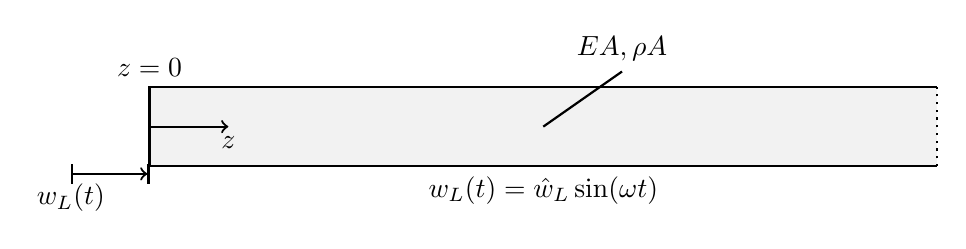
\begin{tikzpicture}
        \draw[thick, fill=gray!10] (10,0) -- node [midway, below] {$w_L (t) = \hat{w}_L \sin(\omega t)$} (0,0) -- (0,1) node[above] {$z=0$} -- (10,1) ;
        \draw[thick, dotted] (10,0) -- (10,1);
        %\draw[thick, ->] (10,0.5) -- (11,0.5);
        \draw[thick, ->] (0,0.5) -- (1,0.5) node[left, below] {$z$} ;
        \draw[thick, |->|] (-1,-0.1) node[below] {$w_L (t)$} -- (0,-0.10);
        \draw[thick] (5,0.5) -- (6,1.2) node[above] {$EA,\rho A$};
    \end{tikzpicture}
\end{figure}


Am Anfang $(t=0)$ ist er undeformiert und in Ruhe. Lösen Sie diese Aufgabe, indem Sie auf dem gedanklich über den Rand verlängerten Stab eine nach rechts laufende Welle annehmen, welche genau die vorgegebene Randbewegung erzeugt. Interpretieren Sie die Parameter dieses Verlaufs physikalisch, Stichwort ``Wellenlänge".
}

\begin{solution}
    
    \begin{align*}
        \intertext{Aus dem D'alembertschen Wellenansatz mit $t = 0$}
        &w_0(z) = \Psi(z) + \Phi(z)
        &\dot{w_0}(z) = c\Psi^{'}(z)-c\Psi^{'}(z)
        \intertext{folgt:}
        &\Psi(z) = C_1 \cos(\kappa z) + C_2 \sin(\kappa z)
        &\Phi(z) = R_1 \cos(\kappa z) + R_2 \sin(\kappa z)
    \end{align*}
\end{solution}

\question{Berechnen Sie das Reflektionsverhalten diskreter Elemente am Rand: Feder, Dämpfer und Masse.
\begin{figure}[h]
    \centering
    \begin{tikzpicture}

    \end{tikzpicture}
\end{figure}

\input{fig_tikz/discrete_boundary_impedance}

Nehmen Sie dazu eine einfallende nach links laufende Welle $w_{ein}(z,t) = C_1 \cos(kz+\omega t)$ an und berechnen Sie die reflektierende Welle $w_{ref}(z,t)=R_1\cos(kz-\omega t) + R_2 \sin(kz-\omega t)$.
}\\[2em]

\fbox{Hinweis ($z=0$):}
\begin{tasks} (3)
    \task[] $kw = EAw'$
    \task[] $c\dot w = (EA)w'$
    \task[] $m\ddot w = (EA)w'$
    \task[] Feder-RB
    \task[] Dämpfer-RB
    \task[] Masse-RB
\end{tasks}

\fbox{
    \begin{minipage}[t]{\textwidth}
        Hinweis: Der Punkt steht für die Ableitung nach der Zeit $t$, \\der Apostroph für die Ableitung nach der räumlichen Koordinate $z$.
    \end{minipage}}

\begin{solution}
        \intertext{Ableitungen der Funktion $w$:}
        \begin{align*}
            \dot{w} &= -C_1 \omega \sin(\kappa z + \omega t) + C_2 \omega \cos(\kappa z + \omega t) \\
                    & R_1 \omega \sin(\kappa z - \omega t) - R_2 \omega \cos(\kappa z - \omega t) \\
            ddot{w} &= - C_1 \omega^2 \cos(\kappa z + \omega t) - C_2 \omega^2 \sin(\kappa z + \omega t) \\
                    & -R_1 \omega^2 \cos(\kappa z - \omega t) - R_2 \omega^2 \sin(\kappa z - \omega t) \\
            w^{'} &= -C_1 \kappa \sin(\kappa z + \omega t) + C_2 \kappa \cos(\kappa z + \omega t) \\
                  & -R_1 \kappa \sin(\kappa z - \omega t) + R_2 \kappa \cos(\kappa z - \omega t)
        \end{align*}

        Schrittweise Berechnung der Reflektion: \\
        1\) Anfangsbedingung: $z=0$ \\
        2\) Ausklammern der Sinus- und Cosinus-Ausdrücke (am besten in Matrixform)\\
        3\) Aus den erhaltenen Koeffizienten der Sinus- und Cosinusfunktionen kann nun nach $R_1$ und $R_2$ umgestellt werden.
            Dabei ergibt sich $R_1$ aus den Koeffizienten des Kosinus und $R_2$ aus den Sinuskoeffizienten.\\

        Feder:
        \begin{align*}
        0 &= kw - EA  w^{'}\\
        R_1 &= \frac{C_1 {(EA)}^2 \kappa^2 - C_1 k^2 + 2C_2 (EA) k \kappa}{{(EA)}^2 \kappa^2 + k^2}\\
        R_2 &= \frac{2C_1 (EA) k \kappa - C_2 {(EA)}^2 \kappa^2 + C_2 k^2}{{(EA)}^2 \kappa^2 + k^2}
        \end{align*}
        Dämpfer:
        \begin{align*}
        0 &= c \dot{w} - EA  w^{'}\\
        R_1 &= \frac{C_1 (EA) \kappa - C_1 c w}{(EA) \kappa + cw}\\
        R_2 &= \frac{-C_2 (EA) \kappa + C_2 cw}{(EA) \kappa + cw}
        \end{align*}
        Masse:
        \begin{align*}
        0 &= m \ddot{w} - (EA) w^{'}\\
        R_1 &= \frac{C_1 {(EA)}^2 \kappa^2 - C_1 m^2 \omega^4 - 2C_2 (EA) \kappa m \omega^2}{{(EA)}^2 \kappa + m^2 \omega^4}\\
        R_2 &= \frac{-2C_1 (EA) \kappa m \omega^2 - C_2 {(EA)}^2 \kappa^2 + C_2 m^2 \omega^4}{{(EA)}^2 \kappa + m^2 \omega^4}
    \end{align*}
\end{solution}

\question{Resonant Column}
TODO Dominik Kern

\vspace{1cm}

\begin{tikzpicture}
\draw[thick, fill=black!10!white] (-0.2, 0) rectangle (0.2, 3.0);
\draw[thick, fill=black!20!white] (-0.5, 3) rectangle (0.5, 3.5);
\draw(1, 3.2) node[right] {$J$};
\draw(1, 1.5) node[right] {$G,I,\rho$};
\draw (0, 0) pic [rotate=90, scale=0.5] {DKbase};
\draw[<->, thin] (-0.4, 0) -- node[left] {$l$} (-0.4, 3);
\draw[thin] (0.1, 1.0) -- (1.0, 1.5);
\draw[thin] (0.4, 3.3) -- (1.1, 3.2);
\end{tikzpicture}



		   \subsection{Elastodynamik (3D)}
		   \question{Wellenreflektion} 
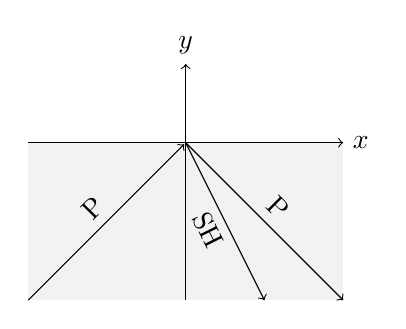
\begin{tikzpicture}
 \fill[black!5!white] (-2,0) rectangle (2,-2);
 \draw[->] (-2,0 ) -- (2,0) node[right] {$x$};
 \draw[->] ( 0,-2 ) -- (0,1) node[above] {$y$};
 \draw[->] (-2,-2) -- node[above, sloped] {P} (-0.02,-0.02);
 \draw[->] (0,0) -- node[below, sloped] {SH} (1, -2);
 \draw[->] (0,0) -- node[above, sloped] {P} (2, -2);
\end{tikzpicture}


In einem linear elastischen, isotropen Kontinuum Elastizitätsmodul $E$ und Querkontraktionszahl $\nu$ trifft eine ebene P-Welle
\begin{equation*}
    \mathbf{u}_1(\mathbf{r},t)=\mathbf{n}_1 A_1 \cos\bigl(\kappa_1 (\mathbf{n}_1\cdot \mathbf{r}-c_\mathrm{P}t)\bigr) 
    \quad \text{mit} \quad
    \mathbf{u}=[u_1,v_1,w_1]^\mathrm{T}
    \quad \text{und} \quad
    \mathbf{r}=[x,y,z]^\mathrm{T}
\end{equation*}
auf einen freien Rand. Die entsprechende Randbedingung lautet
\begin{equation*}
    \sigma_{xy}(\mathbf{r}_\mathrm{R},t) = \sigma_{yy}(\mathbf{r}_\mathrm{R},t) = 0
    \quad \text{mit} \quad
    \mathbf{r}_\mathrm{R}=[x,0,z]^\mathrm{T}. 
\end{equation*}
Die Ausbreitungsrichtung $\mathbf{n}_1=[\sin\alpha_1, \cos\alpha_1, 0]^\mathrm{T}$, Amplitude $A_1$ und Wellenzahl $\kappa_1$ der einfallenden Welle sind vorgegeben.
Gesucht sind die Darstellungen der reflektierten Wellen
\begin{align*}
    \mathbf{u}_2(\mathbf{r},t) &= \mathbf{n}_2 A_2 \cos\bigl(\kappa_2 (\mathbf{n}_2\cdot \mathbf{r}-c_\mathrm{P}t)\bigr)
    \quad \text{mit} \quad
    \mathbf{n}_2=[\sin\alpha_2,\, -\cos\alpha_2,\, 0]^\mathrm{T}, \\
    \mathbf{u}_3(\mathbf{r},t) &= \mathbf{e}_z\times\mathbf{n}_3 A_3 \cos\bigl(\kappa_3 (\mathbf{n}_3\cdot \mathbf{r}-c_\mathrm{S}t)\bigr)
    \quad \text{mit} \quad 
    \mathbf{n}_3=[\sin\beta,\, -\cos\beta,\, 0]^\mathrm{T}
    \quad \text{und} \quad
    \mathbf{e}_z=[0,0,1]^\mathrm{T}.
\end{align*}

 geg/ges.: TODO siehe V06aufgabe.pdf (handschriftlich), vormals V07aufgabe.pdf

\begin{minipage}[t]{\textwidth}
    geg.:
    \begin{tasks} (2)
        \task[] elastisches Kontinuum:
        \task[] %Platzhalter für Struktur im Dokument
        \task[] $\Lambda = \frac{E v}{(1-2v)(1+v)}$
        \task[] $\mu = \frac{E}{2(1+v)}$
        \task[] einfallende P-Welle:
        \task[] %Platzhalter
        \task[] $w_1 = A_1 n_1 \exp(i \kappa_1(n_1 r-c_p t))$ 
        \task[] mit: $n_1 = 
                \begin{bmatrix}
                    \sin(\alpha_1) \\
                    \cos(\alpha_1) \\
                    0
                \end{bmatrix}$ und $r = \begin{bmatrix}
                    x \\ y \\ 0
                \end{bmatrix}$
        \task[] spannungsfreier Rand $y = 0$:
        \task[] %Platzhalter
        \task[] $\sigma_{xy} (x,0,z,t) = \sigma_{yy} (x,0,z,t) = 0$
    \end{tasks}
\end{minipage}

\begin{minipage}[t]{.49\linewidth}
    ges.:
    \begin{tasks}

    \end{tasks}
\end{minipage}

\begin{solution}
    Phasen der einfallenden P-Welle $P_{in}$, der reflektierten P-Welle $P_{ref}$ und der reflektierten SH-Welle $S_{ref}$:
    \begin{align*}
            &\phi_{P_{in}} = \textit{i} \cdot \kappa_P (x \sin(\alpha) + y \cos(\alpha) - c_P t) \\
            &\phi_{P_{ref}} = \textit{i} \cdot \kappa_P (x \sin(\alpha) - y \cos(\alpha) - c_P t) \\
            &\phi_{S_{ref}} = \textit{i} \cdot \kappa_S (x \sin(\beta) - y \cos(\beta) - c_S t)
    \end{align*}

    komplexe Darstellung der Wellenausbreitung aller drei Wellen:

    \begin{align*}
        &P_{in_{complex}} = \hat{A_{P_{in}}} \exp(\phi_{P_{in}}) \\
        &P_{ref_{complex}} = \hat{A_{P_{ref}}} \exp(\phi_{P_{ref}}) \\
        &S_{ref_{complex}} = \hat{A_{S_{ref}}} \exp(\phi_{S_{ref}})
    \end{align*}

    Verschiebungen in Richtung (x,y):

    \begin{align*}
        &x_{P_{in}} = P_{in_{complex}} \sin(\alpha) \\
        &x_{P_{ref}} = P_{ref_{complexx}} \sin(\alpha) \\
        &x_{S_{ref}} = S_{ref_{complex}} \cos(\beta) \\
        \\
        &y_{P_{in}} = P_{in_{complex}} \cos(\alpha) \\
        &y_{P_{ref}} = - P_{ref_{complex}} \cos(\alpha) \\
        &y_{S_{ref}} = S_{ref_{complex}} \sin(\alpha)
    \end{align*}

    Spannungen $ \sigma_{xy}$ und $\sigma_{yy}$, die relevant für die Reflexion sind:

    \begin{align*}
        &\sigma_{xy_{Pin}} = \mu (\frac{\delta x_{P_{in}}}{\delta y} + \frac{\delta y_{P_{in}}}{\delta x}) \\
        &\sigma_{xy_{Pref}} = \mu (\frac{\delta x_{P_{ref}}}{\delta y} + \frac{\delta y_{P_{ref}}}{\delta x}) \\
        &\sigma_{xy_{Sref}} = \mu (\frac{\delta x_{S_{ref}}}{\delta y} + \frac{\delta y_{S_{ref}}}{\delta x}) \\
        \\
        &\sigma_{yy_{Pin}} = (2\mu + \Lambda) \frac{\delta y_{P_{in}}}{\delta y} + \Lambda \frac{\delta x_{P_{in}}}{\delta x} \\
        &\sigma_{yy_{Pref}} = (2\mu + \Lambda) \frac{\delta y_{P_{ref}}}{\delta y} + \Lambda \frac{\delta x_{P_{ref}}}{\delta x} \\
        &\sigma_{yy_{Sref}} = (2\mu + \Lambda) \frac{\delta y_{S_{ref}}}{\delta y} + \Lambda \frac{\delta x_{S_{ref}}}{\delta x} \\
    \end{align*}

    Auswertungen der Spannungen am Rand:

    \begin{align*}
        &\sigma_{xy_{Rand}} &&= \frac{\sigma_{xy_{Pin}} \exp(-\phi_{P_{in}})}{i} + \frac{\sigma_{xy_{Pref}} \exp(-\phi_{P_{ref}})}{i}
                            + \frac{\sigma_{xy_{Sref}} \exp(-\phi_{S_{ref}})}{i} \\
                            &&= \mu (\hat{A_{P_{in}}} \kappa_P \sin(2\alpha) - \hat{A_{P_{ref}}} \kappa_P \sin(2 \alpha) 
                            - \hat{A_{S_{ref}}} \kappa_S \cos(2\beta))\\
        &\sigma_{yy_{Rand}} &&= \frac{\sigma_{yy_{Pin}} \exp(-\phi_{P_{in}})}{i} + \frac{\sigma_{yy_{Pref}} \exp(-\phi_{P_{ref}})}{i}
                            + \frac{\sigma_{yy_{Sref}} \exp(-\phi_{S_{ref}})}{i} \\
                            &&= \hat{A_{P_{in}}} \kappa_P (\Lambda + 2 \mu \cos[2](\alpha)) + \hat{A_{P_{ref}}} \kappa_P (\Lambda + 2 \mu \cos[2](\alpha))
                            - \hat{A_{S_{ref}}} \kappa_S \mu \sin(2\beta)
    \end{align*}

    Die Amplituden der reflektierten Wellen sind beide winkelabhängig. Um diese zu berechnen, löst man nun die Randbedingungen nach 
    $A_{P_{ref}}$ und $ A_{S_{ref}}$ auf. Das Ergebnis lautet, wie folgt:

    \begin{align*}
        &A_{P_{ref}} = \frac{
            A_{P_{in}} (- \Lambda \cos(2 \beta) + \mu \sin(2\alpha)\sin(2\beta) - 2 \mu \cos[2](\alpha) \cos(2\beta))
        }{
            \Lambda \cos(2 \beta) + \mu \sin(2 \alpha) \sin(2\beta) + 2 \mu \cos[2](\alpha) \cos(2 \beta)
        } \\
        &A_{S_{ref}} = \frac{
            2 A_{P_{in}} \kappa_P (\Lambda \sin(2 \alpha) + \mu \sin(2 \alpha) + \frac{\mu \sin(4 \alpha)}{2})
        }{
            \kappa_S (\Lambda \cos(2 \beta) + \mu \cos(2 \beta) + \mu \cos(2\alpha - 2\beta) )
        }\\
    \end{align*}
\end{solution}
		
		\newpage
		\section{Praktische Anwendung}
		   \subsection{Kennwertermittlung}
		   TODO Dominik Kern

\bigskip

Schubmodul statisch (Scher-, Torsionsversuch) und dynamisch (Wellengeschwindigkeit, Verweis auf Schwingungen) 






		   \subsection{Konstruktionskriterien}
		   Erdbebenersatzkraft anhand des Bemessungsspektrums.
TODO Aufgabe V09aufgabe.pdf (handschriftlich)

	
	\end{questions}

\end{document}
